\documentclass[acmsmall,screen]{acmart}

\bibliographystyle{ACM-Reference-Format}
\citestyle{acmauthoryear}

%% Some recommended packages.
\usepackage{booktabs}   %% For formal tables:
                        %% http://ctan.org/pkg/booktabs
\usepackage{subcaption} %% For complex figures with subfigures/subcaptions
                        %% http://ctan.org/pkg/subcaption

\usepackage[english]{babel}
\usepackage{bookmark}
\usepackage[utf8]{inputenc}
\usepackage[T1]{fontenc}
% \usepackage{lmodern}
\usepackage{xspace}
\usepackage{fancyhdr}
\usepackage{tcolorbox}

% Haskell code snippets and useful shortcuts
\usepackage{minted}
\setminted[haskell]{escapeinside=@@}
\newcommand{\hs}{\mintinline{haskell}}
\newcommand{\subhs}{\mintinline[fontsize=\small]{haskell}}
\newcommand{\cmd}[1]{\textsf{\color[rgb]{0,0,0.5} #1}}
\newcommand{\teq}{\smaller $\sim$}
\newcommand{\ghci}{$\lambda$>}
\newcommand{\defeq}{\stackrel{\text{def}}{=}}
\newcommand{\dollar}{{\color[rgb]{0.40,0.40,0.40} \$}}
\newcommand{\std}[1]{{\color[rgb]{0,0.3,0} #1}}
\newcommand{\blk}[1]{{\color[rgb]{0,0,0} #1}}
\newcommand{\blu}[1]{{\color[rgb]{0,0,1.0} #1}}

% Questions and tasks
\newcommand{\q}[2]{\textbf{\color{blue} Question #1:} #2}
\newcommand{\todo}[2]{[\textbf{\color{red} #1:} #2]}

% Abbreviations for projects
% \newcommand{\Dune}{\textsc{Dune}\xspace}
% \newcommand{\Haxl}{\textsc{Haxl}\xspace}

\begin{document}

%% Title information
\title{Formal Verification of Spacecraft Control Programs}

\author{Georgy Lukyanov}
\affiliation{
  \institution{Newcastle University}
  \country{United Kingdom}
}
\email{g.lukyanov2@ncl.ac.uk}
\author{Andrey Mokhov}
\affiliation{
  \institution{Newcastle University}
  \country{United Kingdom}
}
\email{andrey.mokhov@ncl.ac.uk}
\author{Jakob Lechner}
\affiliation{
  \institution{RUAG Space GmbH}
  \country{Austria}
}
\email{jakob.lechner@gmx.net}

% Don't forget \thispagestyle{firstpagestyle} after \maketitle
% \fancypagestyle{firstpagestyle}
% {
%    \fancyhf{}
%    \renewcommand{\headrulewidth}{0.2pt}
%    \fancyhead[C]{Under review, feedback is sought}
% }

\begin{abstract}
Verification of correctness of control programs is an essential task
in the development of space electronics; it is difficult and typically
outweighs design and programming tasks in terms of development hours.
This experience report presents a verification approach designed to help
spacecraft engineers reduce the effort required for formal verification of
low-level control programs executed on custom hardware.

% The approach uses a
% metalanguage to describe the semantics of a program as a state transformer,
% which can be compiled to multiple targets for testing, formal verification, and
% code generation. The metalanguage is embedded in Haskell, providing a way to
% prove some properties at the type level, which can shorten the feedback loop
% and further increase the productivity of engineers.

The verification approach is demonstrated on an industrial case study.
We present REDFIN, a processing core used in space missions, and its formal
semantics expressed using the proposed metalanguage for state transformers,
followed by examples of verification of simple control programs.

\keywords{formal verification, instruction set architecture, functional
programming, domain-specific languages.}
\end{abstract}

\keywords{}

\maketitle
% \thispagestyle{firstpagestyle}

\input{1-intro}
\section{The REDFIN architecture overview\label{sec-redfin}}
% For many spacecraft subsystems integrated circuits are required to perform control
% tasks or simple data processing. Typically, these integrated circuits are realised
% with FPGAs (Field Programmable Gate Arrays) due to their flexibility and lower
% costs compared to ASIC (Application-Specific Integrated Circuit) development \&
% fabrication. Since FPGAs can be used to implement arbitrary circuit functions
% including processor cores, it is possible to perform tasks both in hardware and
% in software. However, modern space-qualified FPGAs, which can withstand radiation
% in Earth orbit or deep space, have a limited amount of programmable resources.
% Therefore, it is often not feasible to implement a fully-fledged processor system
% in such an FPGA next to the mission-specific circuitry.

Many spacecraft subsystems rely on integrated circuits to perform control tasks
or simple data processing. Typically, these integrated circuits are realised
with Field Programmable Gate Arrays (FPGAs) benefiting from their flexibility
and low cost. Modern space-qualified FPGAs that can withstand radiation in Earth
orbit or deep space have a limited amount of programmable resources, and it is
often not feasible to implement a fully-fledged processor system in such an FPGA
next to the mission-specific circuitry.
The REDFIN instruction set was developed to address this issue and meet the
following goals: (i)~simple instruction set with a small hardware footprint,
(ii)~reduced complexity to support formal verification of programs, and
(iii)~deterministic real-time behaviour.

\subsection{REDFIN instruction set and microarchitecture}

REDFIN instructions have a fixed width of 16 bits.
The instruction set is based on a register-memory architecture, i.e.
instructions can fetch their operands from registers as well as directly from the
memory. This architecture favours a small register set, which minimises the hardware
footprint of the processing core. Furthermore, the number of instructions in a
program is typically smaller in comparison to traditional load/store architectures
where all operands have to be transferred to registers before any operations can
be performed. There are 47 instructions of the following types:

\begin{itemize}
\item{Load/store instructions for moving data between registers and memory, and
loading of immediate values.}
\item{Integer and fixed-point arithmetic operations.}
% In the latter
% case the number of fractional bits can be adjusted by a processor register.
\item{Bitwise logical and shift operations.}
\item{Control flow instructions and comparison operations.}
\item{Bus access instructions for read \& write operations on an AMBA AHB bus
(not covered in this paper).}
\end{itemize}

The REDFIN processing core fetches instruction and data words from a small and fast
on-chip SRAM. This only allows for execution of simple programs, however, it also
eliminates the need to implement caches and thus removes a source of non-determinism of
conventional processors. High performance is not one of the main goals, hence the
core is not pipelined and does not need to resolve data/control hazards or
perform any form of speculative execution. These properties greatly simplify
worst case execution time analysis.

\subsection{Requirements for formal verification}

Verification of \emph{functional correctness} of REDFIN programs, as defined by a
requirement specification, clearly is an essential task for the development of space
electronics. There are also important \emph{non-functional requirements}, such as
worst case execution time and energy consumption, which rely on the implementation
guarantees provided by the processing core. To reduce verification complexity,
the REDFIN core only allows to execute a single subroutine whose execution is triggered
by a higher-level controller in the system. The implementation guarantees that
concurrent bus accesses to the processor registers or memory do not affect
the subroutine execution time. Furthermore, the processor does not implement
interrupt handling. All these measures are taken to provide real-time
subroutine execution guarantees and make the verification of non-functional
properties feasible. % within the presented verification framework.

Despite these restrictions the REDFIN core has already proven its effectiveness for
simple control tasks and arithmetic computations as part of an antenna pointing unit
for satellites. Nevertheless, verification can be difficult and time-consuming,
even for small and simple programs. Verification activities, following engineering
standards for space electronics, typically outweigh programming and design tasks by a
factor of two in terms of development hours. Usually verification is performed via
program execution on an instruction set simulator or a hardware model of the processor.
Manually deriving test cases from the specification is cumbersome and error-prone
and simulation times can become prohibitively long with a large number of tests that
are often needed to reach the desired functional and code coverage. Formal verification
methods can prove that a program satisfies certain properties for all possible
test cases and are therefore immensely valuable for completing the verification
with superior efficiency and quality.

\input{3-model-state}
\section{Formal verification\label{sec-verification}}
This section presents the formal verification framework developed on top of
the REDFIN semantic core (\S\ref{sec-transformer}) demonstrating the following
steps of the workflow:

\begin{itemize}
    \item Develop programs in low-level REDFIN assembly, and in a high-level
    typed language embedded in Haskell.
    \item Test REDFIN programs on concrete input values.
    \item Define functional correctness and worst case execution time properties
    in the SBV property language.
    \item Verify the properties or obtain counterexamples.
\end{itemize}

\noindent
Consider the following simple spacecraft control task.

\begin{tcolorbox}
Let $t_1$ and $t_2$ be two different time points (measured in ms),
and $p_1$ and $p_2$ be two power values (measured in mW).
Calculate the estimate of the total energy consumption during this period
using linear approximation, rounding down to the nearest integer:
\[
\textit{energyEstimate}(t_1, t_2, p_1, p_2) = \left\lfloor \frac{|t_1 - t_2| * (p_1 + p_2)}{2} \right\rfloor.
\]
\end{tcolorbox}

\noindent
This task looks too simple, but in fact it has a few pitfalls that,
if left unattended, may lead to the failure of the space mission. Examples
of subtle bugs in seemingly simple programs leading to a catastrophe include 64-bit
to 16-bit number conversion overflow causing the destruction of Ariane~5
rocket~\cite{bug-rocket} and the loss of NASA's Mars orbiter due to incorrect
unit conversion~\cite{NASA:1999:Mars}. Let us develop and verify
a REDFIN program for this task.

% \subsubsection{Writing the program}
We can write programs in the untyped REDFIN assembly, or in a typed higher-level
expression language. The former allows engineers to hand-craft highly optimised
programs under tight resource constraints, while the latter brings type-safety
and faster prototyping. We start with the high-level approach and define an
expression that can be used both as a Haskell function and a high-level REDFIN
expression:

% Using Haskell's polymorphism, we can

\begin{minted}[fontsize=\small]{haskell}
energyEstimate :: Integral a => a -> a -> a -> a -> a
energyEstimate t1 t2 p1 p2 =
    abs (t1 - t2) * (p1 + p2) `div` 2
\end{minted}

\noindent
Thanks to polymorphism, we can treat \hs{energyEstimate} both as a numeric
function, and as an abstract syntax tree that can be \emph{compiled} into a
REDFIN assembly \hs{Script}. Due to the lack of space we omit the implementation
of \hs{Script}, but one can think of it as a restricted version
of the \hs{Redfin} state transformer, which we use to write \emph{programs that
can manipulate the processor state only by executing instructions}, e.g. the
only way to set the \hs{Overflow} flag is to execute an arithmetic instruction
that might cause an overflow.

\begin{minted}[xleftmargin=10pt,fontsize=\small]{haskell}
energyEstimateHighLevel :: Script
energyEstimateHighLevel = do
  let t1    = read (IntegerVariable 0)
      t2    = read (IntegerVariable 1)
      p1    = read (IntegerVariable 2)
      p2    = read (IntegerVariable 3)
      temp  = Temporary 4
      stack = Stack 5
  compile r0 stack temp (energyEstimate t1 t2 p1 p2)
  halt
\end{minted}
\label{energyEstimateHighLevel}

\noindent
Here the type \hs{IntegerVariable} is used to statically distinguish between integer
and fixed-point numbers, \hs{Temporary} to mark temporary words, so they cannot
be mixed with inputs and outputs, and \hs{Stack} to denote the location of the
stack pointer. The~\hs{let} block declares six adjacent memory addresses: four
input values $\{t_1, t_2, p_1, p_2\}$, a temporary word and a stack pointer.
We~\hs{compile} the high-level expression \hs{energyEstimate} into the assembly
language by translating it to a sequence of REDFIN instructions. The first
argument of the~\hs{compile} function holds the register~\hs{r0} which contains
the estimated energy value after the program execution.

% \subsubsection{Simulating the program}
We can run symbolic simulation for 100 steps, initialising the program and data
memory of the processor using the function \hs{simulate} defined above and a
helper function \hs{boot}.

\begin{minted}[xleftmargin=10pt,fontsize=\small]{haskell}
main = do
  let dataMemory = [10, 5, 3, 5, 0, 100]
      finalState = simulate 100 $
        boot energyEstimateHighLevel dataMemory
  printMemoryDump 0 5 (memory finalState)
  putStrLn $ "R0: " ++ show
             (readArray (registers finalState) r0)
\end{minted}

\noindent
As the simulation result we get a \hs{finalState}. We inspect it by
printing relevant components: the values of the first six memory cells, and the
result of the computation located in the register~\hs{r0}. Note that the stack
pointer (cell 5) holds 100, as in the initial state, which means the stack is empty.

\begin{minted}[frame=single, fontsize=\small]{text}
Memory dump: [10, 5, 3, 5, 5, 100]
R0: 20
\end{minted}

Simulating programs with specific inputs is useful for diagnostic and test, but
SMT solvers allow us to verify the correctness for \emph{all valid input
combinations}. To demonstrate this, let us discover a problem in our energy
estimation program. Consider the following correctness property.

% \subsubsection{Verifying the program}
% The project lead engineer defined a set of functional requirements for the
% energy monitoring subsystem. The software engineering team received the
% specification, implemented the energy monitoring subroutines, and started the
% verification. One of the requirements is as follows.

\begin{tcolorbox}
Assuming that values $p_1$ and $p_2$ are non"/negative integers, the energy
estimation subroutine must always return a non-negative integer value.
\end{tcolorbox}

To check that the program meets this requirement, we translate
\hs{energyEstimateHighLevel} into an SMT formula,
and formulate the corresponding theorem:

\begin{minted}[fontsize=\small]{haskell}
theorem = do
  t1 <- forall "t1" -- Initialise symbolic variables
  t2 <- forall "t2"
  p1 <- forall "p1"
  p2 <- forall "p2" -- And then add constraints:
  constrain $ p1 .>= 0 &&& p2 .>= 0
  -- Initialise the data memory with symbolic variables:
  let dataMemory = [t1, t2, p1, p2, 0, 100]
      finalState = simulate 100
        (boot energyEstimateHighLevel dataMemory)
      result = readArray (registers finalState) r0
      halted = readArray (flags finalState) (flagId Halt)
  return $ halted &&& result .>= 0
       &&& result .== energyEstimate t1 t2 p1 p2
\end{minted}

\noindent
We extract the computed result and the value of the flag \hs{Halt} from the
\hs{finalState}, and then assert that the processor has halted, the result is
non-negative, and is equal to that computed by the high-level Haskell expression
\hs{energyEstimate}.
The resulting SMT formula can be checked by Z3 in
3.0s\footnote{We use a laptop with 2.90GHz Intel Core i5-4300U processor, 8GB
RAM (3MB cache), and the SMT solver Z3 version 4.5.1 (64-bit).}:

\begin{minted}[frame=single,fontsize=\small]{text}
> proveWith z3 theorem
Falsifiable. Counter-example:
  t1 = 5190405167614263295 :: Int64
  t2 =                   0 :: Int64
  p1 =  149927859193384455 :: Int64
  p2 =  157447350457463356 :: Int64
\end{minted}

%TODO: Can we obtain a simpler counterexample using SBV optimisation?
\noindent
Z3 has found a counterexample demonstrating that the program does not
satisfy the above property. Indeed, the expression evaluates to a negative
value on the provided inputs due to an \emph{integer overflow}. We therefore
refine the property:

\begin{tcolorbox}
According to the spacecraft power system specification, $p_1$ and $p_2$ are
non"/negative integers not exceeding 1W. The time is measured
from the mission start, hence $t_1$ and $t_2$ are non-negative and do not exceed
the time span of the mission, which is 30 years. Under these assumptions,
the energy estimation subroutine must return a non-negative integer value.
\end{tcolorbox}

\noindent
We need to modify time and power constraints accordingly:
% \footnote{We are not absolutely
% precise here. We do not distinguish between regular and leap years, and use
% a conservative upper bound of 366 days per year.}

\begin{minted}[xleftmargin=10pt,fontsize=\small]{haskell}
constrain $ p1 .<= toMilliWatts   ( 1 :: Watt)
        &&& t1 .<= toMilliSeconds (30 :: Year)
        &&& t1 .>= 0 &&& t2 .>= 0 &&& ... -- etc.
\end{minted}

\noindent
Rerunning Z3 produces the desired \textsf{QED} outcome in 4.8s.

The refinement has rendered the integer overflow impossible;
in particular, \hs{abs} can never be called with~$-2^{63}$
within the mission parameters. Such guarantee fundamentally requires
solving an SMT problem, even if it is done at the type level, e.g. using
\emph{refinement types}~\cite{vazou2014refinement}.

% \subsubsection{Checking program equivalence}
The statically typed high-level expression language is very convenient for
writing REDFIN programs, however, an experienced engineer can often find a way
to improve the resulting code. In some particularly resource-constrained situations,
a fully hand-crafted assembly code may be required. As an example, a direct
unoptimised translation of the \hs{energyEstimate} expression into assembly uses
79 instructions, most of them for \hs{Stack} manipulation.
On the other hand, it is not difficult to write a low-level assembly program that
computes the result using only 9 instructions:

\begin{minted}[xleftmargin=10pt,fontsize=\small]{haskell}
energyEstimateLowLevel :: Script
energyEstimateLowLevel = do
    let { t1 = 0; t2 = 1; p1 = 2; p2 = 3 }
    ld r0 t1
    sub r0 t2
    abs r0
    ld r1 p1
    add r1 p2
    st r1 p2
    mul r0 p2
    sra_i r0 1
    halt
\end{minted}
\label{energyEstimateLowLevel}

\noindent
To support the development of hand-crafted code, we use Z3 to \emph{check the
equivalence of REDFIN programs} by verifying that they produce
the same output on all valid inputs. This allows an engineer to
optimise a high-level prototype and have a guarantee that no bugs were
introduced in the process. The corresponding \hs{equivalence} check takes 11.5s.
% (on 52 SMT clauses)

% \begin{minted}[frame=single,fontsize=\small]{text}
% > proveWith z3 equivalence
% Q.E.D.
% \end{minted}

% Below we check the \hs{equivalence} of this low-level program with
% \hs{energyEstimateHighLevel} introduced earlier.

% \begin{minted}[xleftmargin=10pt,fontsize=\small]{haskell}
% equivalence = do
%   t1 <- forall "t1"
%   t2 <- forall "t2"
%   p1 <- forall "p1"
%   p2 <- forall "p2"
%   constrain $ p1 .>= 0 &&& p2 .>= 0
%       &&& p1 .<= toMilliWatts   ( 1 :: Watt)
%       &&& p2 .<= toMilliWatts   ( 1 :: Watt)
%       &&& t1 .>= 0 &&& t2 .>= 0
%       &&& t1 .<= toMilliSeconds (30 :: Year)
%       &&& t2 .<= toMilliSeconds (30 :: Year)
%   let memory   = [t1, t2, p1, p2, 0, 100]
%       llState  = simulate 100 (boot energyEstimateLowLevel  memory)
%       hlState  = simulate 100 (boot energyEstimateHighLevel memory)
%       llResult = readArray (registers llState) r0
%       hlResult = readArray (registers hlState) r0
%   return $ llResult .== hlResult
% \end{minted}

% \subsubsection{Program timing analysis}

Every call of the~\hs{executeInstruction} function advances the \hs{clock} field
of the \hs{State} (see Fig.~\ref{fig-types}) by the appropriate number of
cycles, precisely matching the hardware implementation. This allows us to
perform~\emph{best/worst case execution timing analysis} using the
optimisation facilities of SBV and Z3. As an example,
let us determine the minimum and maximum number of clock cycles required for
executing~\hs{energyEstimateLowLevel}. To make this example more
interesting, we modified the semantics of the instruction~\hs{abs} and
added~1~extra clock cycle in case of a negative argument.
% by conditionally performing
% \hs{delay 1} in the state transformer \hs{abs}.

% \begin{minted}{haskell}
% delay :: Clock -> Redfin ()
% delay cycles =
%     Redfin $ \s -> ((), s { clock = clock s + cycles })
% \end{minted}
%TODO: Same can be done about power

\begin{minted}[xleftmargin=10pt,fontsize=\small]{haskell}
timingAnalysis = optimize Independent $ do
  ... -- Initialise and run symbolic simulation
  minimize "Best case"  (clock finalState)
  maximize "Worst case" (clock finalState)
\end{minted}

\noindent
The total delay of the program depends only on the sign of $t_1 - t_2$, thus
the best and worst cases differ only by one clock cycle. The worst case is
achieved when the difference is negative ($t_1 - t_2 = -2$), as shown below.
Z3 finishes in 0.5s.

\noindent
\begin{minipage}{0.53\linewidth}
\begin{minted}[frame=single,fontsize=\small]{text}
Objective "Best case":
Optimal model:
  t1        = 549755813888
  t2        =  17179869184
  p1        =            0
  p2        =            0
  Best case =           12
\end{minted}
\end{minipage}
\begin{minipage}{0.46\linewidth}
\begin{minted}[frame=single,fontsize=\small]{text}
Objective "Worst case":
Optimal model:
  t1         = 65535
  t2         = 65537
  p1         =     0
  p2         =     0
  Worst case =    13
\end{minted}
\end{minipage}

\section{Formal verification in presence of unbounded loops\label{sec-motor-control}}

Many programs targeting REDFIN share the distinctive feature of
the energy estimation program considered in section~\ref{sec-verification},
i.e. the existence of an  upper \emph{bound on execution time},
thanks to the fact that their termination does not
depend on the input data. However, other programs may have loops
which are guarded by termination conditions that involve computation
considering the input parameters of the program, thus making the loop
\emph{unbounded}.

Presence of unbounded loops makes program verification by symbolic execution considerably
harder~\cite[p.~50:20]{SurveySymExec-CSUR18}, since the number of program execution
paths becomes infinite. In this section we apply the developed verification framework
to a larger example of a stepper motor control program and verify one of its essential
safety properties by formulating it as a~\emph{loop invariant} and ensuring that the
invariant holds for every possible state of the loop.

\subsection{Stepper motor control program}

Stepper motors are often deployed as parts of antenna and solar panel pointing units
in space satellites. We consider a program for controlling a motor with
one degree of freedom. The program, given the distance to move the motor and safety
bounds on velocity and acceleration, will

The algorithm~\ref{alg-motor} expects three input
parameters: $dist$ --- the distance to move the motor, $v\_max$ --- the maximal permitted
velocity and $a\_max$ --- the maximal permitted acceleration and computes a series of
speed and velocity values that will be used to move the motor. The conditional statement on
starting in line 9 decides whether to accelerate the motor, to keep it on steady speed or
to decelerate the motor; see~\ref{fig-motor} for example plots of velocity and distance travelled
against time. The spike on the bottom-left of the velocity graph illustrates
the edge covered by the conditional statement on line 18: if the velocity is zero, but the target
distance has not yet been reached, the motor must be moved a bit further.

\begin{algorithm}[h]
  \begin{algorithmic}[1]
\Require {$dist$, $v\_max$, $a\_max$}
\State $s \gets 0$
\State $v \gets 0$
\While {$true$}
  % Compute deceleration distance based on current speed
  \State $decel\_steps\gets \lfloor v / a\_max \rfloor$
  \algorithmiccomment{Compute deceleration distance based on current speed}
  \State $s\_decel \gets a\_max \cdot (decel\_steps + 1) / 2$
  \If {$decel\_steps \cdot a\_max \neq v$}
    \State $s\_decel \gets s\_decel + v$
  \EndIf
  \State {$v\_next = min(v\_max, dist, v + a\_max)$}
  \If {$s + s\_decel + v\_next \leq dist$}
    \State $v \gets v\_next$ \algorithmiccomment{accelerate}
  \ElsIf {$s + s\_decel + v \leq dist$}
    \State $ v \gets v $     \algorithmiccomment{keep speed}
  \Else
     \algorithmiccomment{decelerate}
    \If {$v > decel\_steps \cdot a\_max$}
      \State $v \gets decel\_steps \cdot a\_max$
    \Else
      \State $v \gets v - a\_max$
    \EndIf
  \If {$v = 0$}
    \If {$s \neq dist$}  \algorithmiccomment{accelerate again to reach target}
      % didn't quite reach our target after deceleration
      % => accelerate again
      \State $v \gets min(dist - s, a\_max)$
    \Else
      % reached target
      \State $break$  \algorithmiccomment{terminate execution}
  \EndIf
\EndWhile
\end{algorithmic}
\caption{Motor Control Algorithm\label{alg-motor}}
\end{algorithm}
\begin{figure}[h]
  \centerline{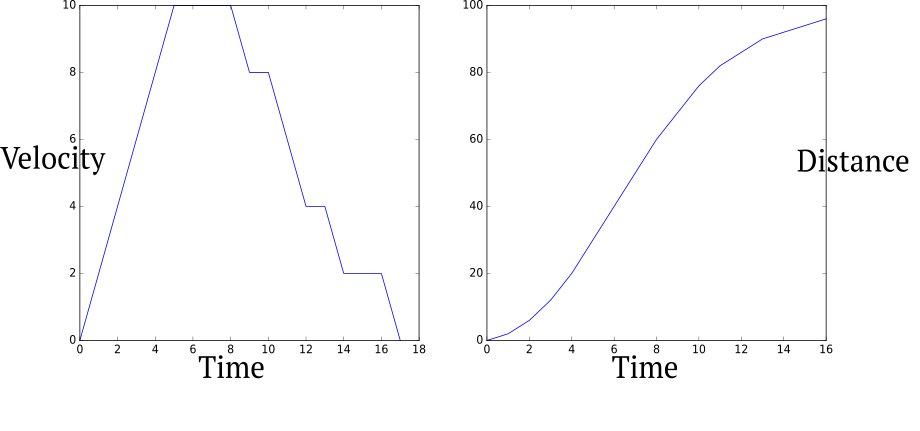
\includegraphics[scale=0.65]{fig/motor_control_graph.pdf}}
  % \vspace{-13mm}
\caption{Velocity ($v$) and distance travelled ($s$) plotted against time\label{fig-motor}}
\Description[Please consult the text of this section for the description]{}
\end{figure}

To be deployed into REDFIN, the algorithm~\ref{alg-motor} must be manually
re-implemented in REDFIN assembly. The resulting assembly program comprises 85 lines of
assembly and closely mirrors the high-level pseudocode. As a sample, consider a fragment of
the program's symbolic execution tree that corresponds to the decision whether to
accelerate, keep speed or decelerate the motor~\ref{fig-sym-tree}.

\begin{figure}[h]
\centerline{
\includegraphics[scale=0.4]{fig/sym-tree-1.pdf}}
\caption{Symbolic execution tree of code fragment with conditional branching\label{fig-sym-tree}}
\Description[Please consult the text of this section for the description]{}
\end{figure}

The decision is based on first estimating the resulting distance travelled using
the next potential value $v\_next$ as velocity and if $dist$ is not covered by that
the motor will be accelerated; otherwise the resulting distance gets estimated
using the current velocity $v$ and in case $v$ is sufficient it is kept as the
velocity; otherwise the motor will be decelerated. The changes of speed may be
also seen from the velocity against time plot~\ref{fig-motor}.


\subsection{Loop invariant verification}

In order to ensure that the motor will not introduce disturbances
and will not lead the whole unit out of its normal mode of operation, the velocity and
acceleration of the motor must be kept in safe limits. This verification condition
is motivated by the correctness requirements of the whole space satellite unit.

More formally, the verification condition means
that in any iteration of the control program loop the values of the
expressions $v$, the velocity, and $\left| v\_next - v \right|$,
the acceleration, must never exceed the parameters $v\_max$ and $a\_max$, respectively.
This property is the loop invariant for the motor control program which
ensures that velocity and acceleration always stay within their safe bounds. We
formalise it as the following predicate that universally quantifies over the
program's inputs and the loop's state:

\begin{tcolorbox}
\LARGE{
\[
  \forall\ v\_max\ a\_max\ v\ v\_next\ s,
  \ v \leq v\_max \land \left| v\_next - v \right| \leq a\_max
\]}
\end{tcolorbox}

\noindent
We will verify the loop invariant by using the verification framework in the
\emph{branching mode}\ref{sec-operation-modes}. While symbolic execution with
merging, which is implemented by the framework's \emph{mergin} mode, allows
for intuitive formulation of properties for whole-program verification and
is very useful for verifying finite programs, as we have
reported in the section~\ref{sec-verification}, in presence of branches guarded
by symbolic values, it suffers from \emph{symbolic non-termination}.
Thus, for verifying the loop invariant, we rely on traditional symbolic execution.

To verify the loop invariant we take the following approach:

\begin{itemize}
  \item Obtain the binary tree-shaped trace by \emph{bounded} symbolic execution
  in \emph{branching} mode
  \item Split the trace into linear paths, thus enumerating all the possible
    execution scenarios
  \item For every path perform the analysis
    \begin{enumerate}
      \item Extract the relevant parts of the state from the \emph{last} node in
            the path, i.e. symbolic expressions stored in
            registers, memory cells or flags
      \item Construct a symbolic expression representing the \emph{property to check},
            which would involve the expressions obtained in the previous step
      \item Extract the \emph{path condition} from the /last/ node in the path
      \item Formulate the \emph{preconditions} of the program
      \item To verify the property in the given path by checking the following
            formula for satisfiability:
              preconditions /\ path constraints /\ ¬ property to check
    \end{enumerate}
    \item  The property holds if and only if for every path the solver returns
           \hs{Unsatisfiable}, i.e. there are no assignments of the variables which
           satisfy the~\emph{negation} of the property to check, considering the
           preconditions and the path condition.
\end{itemize}

This detailed verification algorithms has several parameters that need to be specified:

\begin{itemize}
\item Preconditions on $v\_max$ and $a\_max$
\item Symbolic execution bound, i.e. for how many steps perform the execution. Since the
      body of the loop will always terminate this bound can be calculated in advance.
\end{itemize}

\subsection{Pruning branches}

As illustrated by figure~\ref{fig-sym-tree}, every conditional jump instruction produces
two branches in the symbolic execution tree: the one
where the current path condition is conjoined with the jump's guard and the one where it is
conjoined with the guard's negation. However, if the resulting
conjunction is unsatisfiable, the corresponding branch does not have to be explored
and can be pruned. Thus the symbolic execution engine need to call an SMT solver every
time a conditional jump is encountered to check if the path conditions of the branches
are satisfiable.

Checking satisfiability of execution path is essential to mitigation the path explosion
problem. Pre-condition, when available, is assigned as the initial path condition and thus
will become a subterm of every formula submitted to the solver. Identifying correct preconditions
is essential for verification since they may drastically reduce the number of satisfiable paths
in the symbolic execution tree of the program that is being verified.


Give the preconditions, an example of the execution path, talk about constant folding
and SMT-solving to prove unsatisfiable paths, make a table(?) with results for different
preconditions: number of path, time to solve a path, length of the path maybe.

\subsection{NOTES}

``Pre-conditions, when
available, may be leveraged to reduce the size of the input
data domains and to only generate test inputs that satisfy
the pre-conditions.''


---

\input{6-discussion}
\section{Related Work\label{sec-related}}
There is a vast body of literature available on the topic of formal verification,
including verification of hardware processing cores and low-level software programs.
Our work builds in a substantial way on a few known ideas that we will review in
this section. We thank the formal verification and programming languages
communities and hope that the formal semantics of the REDFIN processing core
will provide a new interesting benchmark for future studies.

We model the REDFIN microarchitecture using a~\emph{monadic state transformer
metalanguage} -- an idea with a long history.
\citet{fox2010trustworthy} formalise the Arm v7 instruction
set architecture in HOL4 and give a careful account to bit-accurate proofs of
the instruction decoder correctness. Later, \citet{kennedy2013coq}
formalised a subset of the x86 architecture in Coq, using monads for instruction
execution semantics, and \textsf{do}-notation for assembly language embedding.
% Both these models are formalised in proof assistants, thus are powered by full
% dependent types, which allow the usage of mechanised program correctness proofs.
\citet{degenbaev2012formal} formally specified the \emph{complete} x86
instruction set -- a truly monumental effort! -- using a custom domain-specific
language that can be translated to a formal proof system. Arm's Architecture
Specification Language (ASL) has been developed for the same purpose to formalise the
Arm v8 instruction set~\cite{reid2016cav}. The SAIL language~\cite{SAIL-lang} has
been designed as a generic language for ISA specification and was used to
specify the semantics of ARMv8-A, \mbox{RISC-V}, and \mbox{CHERI-MIPS}.
Our specification approach is similar to these three works, but we operate on a
much smaller scale of the REDFIN core and focus on verifying whole programs.

Our metalanguage is embedded in Haskell and does not have a rigorous
formalisation, i.e. we cannot prove the correctness of the REDFIN semantics
itself, which is a common concern, e.g. see~\citet{reid2017oopsla}. Moreover, our
verification workflow mainly relies on \emph{automated} theorem proving, rather
than on \emph{interactive} one. This is motivated by the cost of precise proof
assistant formalisations in terms of human resources: automated techniques are
more CPU-intensive, but cause less ``human-scaling issues''~\cite{reid2016cav}.
Our goal was to create a framework that could be seamlessly
integrated into an existing spacecraft engineering workflow, therefore it needed
to have as much proof automation as possible. The automation is achieved by means
of \emph{symbolic program execution}. \citet{Currie2006} applied
symbolic execution with uninterpreted functions to prove equivalence of low-level
assembly programs. The framework we present allows not only proving the
equivalence of low-level programs, but also their compliance with higher-level
specifications written in a subset of Haskell.

% A lot of research work has been done on the design of \emph{typed assembly
% languages}, e.g. see~\cite{Haas:2017:BWU:3140587.3062363}\cite{Morrisett:1999:SFT:319301.319345}.
% The low-level REDFIN assembly is untyped, but the syntactic language of
% arithmetic expressions that we implemented on top of it does have a simple type
% system. In principle, the REDFIN assembly itself may benefit from a richer type
% system, especially one enforcing correct operation with relevant mission-specific
% units of measurement~\cite{Kennedy:1997:RPU:263699.263761}.

Finally, we would like to acknowledge the projects and talks
that provided an initial inspiration for this work: the `Monads to Machine
Code' compiler by \citet{diehl-monads-to-machines}, \mbox{RISC-V} semantics
by~\citet{riscv-semantics}, the assembly monad by~\citet{asm-monad}, and
SMT-based program analysis by \citet{haskell-z3}.

\section*{Acknowledgements}
We would like to thank Vitaly Bragilevsky, Georgi Lyubenov, Neil Mitchell, Charles Morisset,
Artem Pelenitsyn, Danil Sokolov, as well as the three Haskell Symposium
reviewers for their helpful feedback on an earlier version of this paper.

\begin{acks}
\end{acks}

\newpage
\bibliography{refs}
\end{document}